
\documentclass[submit,PRO]{ipsj}
%\documentclass{ipsj}

\usepackage{PROpresentation}
\PROheadtitle{y-n-(x): 情報処理学会プログラミング研究会 発表資料 Y年m月d日}

\usepackage{graphicx}
\usepackage{latexsym}


\def\Underline{\setbox0\hbox\bgroup\let\\\endUnderline}
\def\endUnderline{\vphantom{y}\egroup\smash{\underline{\box0}}\\}
\def\|{\verb|}

\setcounter{巻数}{59}
\setcounter{号数}{1}
\setcounter{page}{1}


\受付{2016}{3}{4}
%\再受付{2015}{7}{16}   %省略可能
%\再再受付{2015}{7}{20} %省略可能
%\再再受付{2015}{11}{20} %省略可能
\採録{2016}{8}{1}




\begin{document}


\title{再帰的ブロック構造を持つ並列プログラムに対する\\
      可逆実行環境}

\etitle{A reversible runtime for parallel programs with recursive blocks}

\affiliate{NUniv}{名古屋大学情報学研究科\\
Graduate school of imformatics, Nagoya University,\\
Furo-cho, Chikusa-ward, Nagoya-city, 464-8601}



\author{池田 崇志}{Takashi Ikeda}{NUniv}[tikeda@sqlab.jp]
\author{結縁 祥治}{Shoji Yuen}{NUniv}[yuen@sqlab.jp]


\begin{abstract}
本論文では,並列に実行されるブロック構造を持つプログラムの実行を解
析することを目的として可逆実行環境の実装を示す.並列プログラムを抽象
機械の3番地コードに変換して実行する.順方向の実行時は逆向き実行に必
要な情報をスタックに保存し,その実行を逆向きに辿る実行環境を実装す
る.この実行環境では,順方向の抽象命令を逆方向の抽象命令に一対一に変
換することで逆向き実行を実現する.

抽象命令の変換による実行環境[T.Ikeda and S.Yuen, 2020] では,並列実
行において抽象機械をPython のmultiprocessing モジュールでフォークす
る抽象命令を実装し,順方向および逆方向において並列実行する実行環境を
示した.

ここでは,実際的なプログラムの構文要素として,ブロック構造,手続き
呼び出し,関数呼び出しを含むように拡張した.Hoey らの手法に従って変
数のスコープを扱うために,各ブロックに名前を付け,参照情報をパスとし
て表し,局所変数を実現する.本研究で新たに提案する方法として抽象命令
生成時に作成する並列ブロックの開始及び終了番地を記録したテーブルを用
いて並列ブロックを起動することにより順方向,逆方向ともに並列の入れ子
構造を実現する.これらの実現手法によって,ブロック構造を持つプログラ
ミング言語に対して単純な抽象機械の実行メカニズムによって逆方向実行が
可能となることを示し,並列プログラムのデバッグのための基盤として提案
する.
\end{abstract}


\begin{jkeyword}
a
\end{jkeyword}

\begin{eabstract}
This paper presents a reversible runtime of simple parallel programs
with blocks.  A program is translated into a sequence of three-address
abstract machine instructions and abstract machines running in
parallel execute the instructions.  The runtime stores the information
of variable updates and program counter jumps associated with process
identifies on stacks in the forward execution. In the backward
execution, the abstract instructions for forward execution are
converted to reverse abstract instructions one-to-one.

In our previous work, we presented a runtime for parallel programs with
flat-fixed structures.  The runtime executes multiple abstract
machines using the multiprocessing module of Python.

This work extends the runtime for practical language features,
including blocks, procedure-call, and function-call. To deal with the
scope of variables in blocks, we assign the path information with
block names following Hoey et.al.  Besides variable paths, the runtime
records the invocation history of parallel blocks as a table to
reverse the invocation of parallel blocks.  We realize parallel nested
structures in both directions.  We illustrate that executing abstract
machines makes bi-directional execution simple even with the recursive
structure of blocks.  We propose them as a foundation for behavioural
analysis such as debugging.

\end{eabstract}

\begin{ekeyword}
a
\end{ekeyword}

\maketitle

%1
\section{はじめに}





%2
\section{関連研究}

本章では並列プログラムに対する逆方向実行について,先行研究によって提案されている手法について説明する.先行研究によって提案されている手法では,whileループやif文,手続き呼び出しのブロックそして並列ブロックを持つような単純なプログラムを対象としている.この対象プログラムに対して逆方向実行に必要な情報を残すための処理を行う.この処理をAnnotationと呼び対象プログラムにAnnotationを適用し逆方向実行に必要な情報を残せる形式にしたプログラムをAnnotatedプログラムと呼ぶ.Annotatedプログラムを実行することによってこのプログラム自体に逆方向実行に必要な情報が書き込まれる.実行されたAnnotatedプログラムをif文やwhile文,手続き呼び出しそして並列ブロックの構造は保持したままでその他の記述順を反転させることでInvertedプログラムが生成され,これを実行することで対象プログラムの実行を逆方向に辿ることができる.

\subsection{対象プログラムの定義}

\begin{figure}[tb]
\setbox0\vbox{
\hbox{$P ::= \epsilon\ |\ S |\ P;P |\ P\ par\ P$}
\hbox{$S ::= skip | X = E\ pa | if\ In\ B\ then\ P\ else\ Q\ end\ pa|$}
\hbox{$\ \ \ \ \ \ \ \ while\ Wn\ B\ do\ P\ end\ pa | $}
\hbox{$\ \ \ \ \ \ \ \ begin\ Bn\ BB\ end |\ call\ Cn\ n\ pa|$}
\hbox{$\ \ \ \ \ \ \ \ runc\ Cn\ P\ end$}
\hbox{$BB\ ::=\ DV\ DP\ P;\ RP\ RV$}
\hbox{$E::=X |\ n |\ (E)|\ E\ Op\ E$}
\hbox{$B::=T|\ F|\ \lnot B |\ (B)|\ E\ ==\ E |\ E > E|\ B \land B$}
\hbox{$DV\ ::= \epsilon |\ var\ X=E\ pa;\ DV$}
\hbox{$DP\ ::= \epsilon |\ proc\ Pn\ n\ is\ P\ end\ pa;\ DP$}
\hbox{$RV\ ::=\epsilon |\  remove\ X=E\ pa;\ RV$}
\hbox{$RP\ ::= \epsilon |\ remove\ Pn\ n\ is\ P\ end\ pa;\ RP$}
}
\centerline{\fbox{\box0}}
\caption{対象プログラムの定義}
\ecaption{definition of language}
\label{fig:Hdef}
\end{figure}


逆方向実行を行う対象のプログラムに対する定義を示す.対象とするプログラムはwhileループ,if文,手続き呼び出しのブロックそして並列ブロックを持つようなプログラムであり\figref{fig:Hdef}のように定義する.



\subsection{Annotatedプログラム}

\figref{fig:Hdef}で定義された対象プログラムに対してAnnotationを行い,Annotatedプログラムを生成しそれを実行する.

\figref{fig:Annf}でAnnotationの適用規則を示す.対象プログラム$P$からAnnotatedプログラム$AP$への変換は変換規則$a(),ann()$に則って行われる.






\figref{fig:Horiginal}のプログラムから\figref{fig:Hannotated}のプログラムがAnnotatedプログラムの変換規則に則って生成される.この時,手続きp1内のステートメントはブロックb1内のブロックb2に存在しているのでこれらのステートメントのパスはb2*b1に変換する.Annotatedプログラムにはそれぞれのステートメントに識別子を書き込むためにスタックAを書き加えている.




\figref{fig:Hannotated}を実行すると\figref{fig:Hexec}のようにプログラム自体にAnnotation及びパスが書き込まれる.\figref{fig:Hexec}では2回目の手続き呼び出しを行ったものであり手続き呼び出しのブロック自体をコピーしそこにAnnotationとパスを書き込んでいる.




\figref{fig:Hinv}に実行されたAnnotated ProgramからInverted Programへの変換規則を示す.\figref{fig:Hinv}のAPやAQはプログラムP,QにAnnotated Programへの変換規則を適用したものである.ASはステートメントSにAnnotated Programへの変換規則を適用したものである.実行されたパス及びAnnotationに逆向き実行に必要な情報が残されておりこの規則に則って作成されたInverted Programを実行することでAnnotated Programの実行を逆順に辿る実行を行う.




\figref{fig:Hexec}の実行されたAnnotatedプログラムを\figref{fig:Hinv}の変換規則に則ってInverted Programへ変換したものが\figref{fig:Hinvprogram}である.Annotationの数字がそのステートメントが実行された順番を表していてAnnotationに書かれている最大の値から始めて一つずつAnnotationに書かれている数字を遡っていくことでAnnotated Programで行った順方向の実行を逆方向に辿る実行を行うことができる.

%3
\section{並列プログラミング言語}

対象とする並列プログラミング言語はwhileループやif文,手続き呼び出しのブロック,関数呼び出しのブロック,および並列ブロックを持つプログラミング言語である.ソースプログラムを抽象機械命令に変換することで抽象機械によって実行する.並列ブロックはparから始まり,各ブロックを$||$の記号で区切り,rapで終わる.

%3.1
\subsection{対象言語の定義}
\label{sec:3.1}

\begin{figure}[tb]
\setbox0\vbox{
\hbox{$P ::= begin\ bn\ BB\ end$}
\hbox{\ \ \ \ \ \ \ $|$ par an $P(\parallel P)^+$ $rap$}
\hbox{\ \ \ \ \ \ \ $|$ $S$}
\hbox{$BB\ ::=\ DV\ DP\ DF\ P(;P)^+\ RV$}
\hbox{$S\ ::=\ skip\ |\  X = E\ |\ if\ C\ then\ P\ else\ P\ fi\ |$}
\hbox{$\ \ \ \ \ \ \ \ \ \  while\ wn\ C\ do\ P\ od\ |\ call\ cn\ a(X?)$}
\hbox{$DV\ ::=\ (var\ X;)^*$}
\hbox{$DP\ ::=\ (proc\ pn\ a(X?)\ is\ P\ end)^*$}
\hbox{$DF\ ::=\ (func\ fn\ b(X?)\ is\ P\ return)^*$}
\hbox{$RV\ ::=\ (remove\ X;)^*$}
\hbox{$E\ ::=\ X\ |\ n\ |\ (E)\ |\ E\ op\ E | \{cn\ b(X?)\}$}
\hbox{$C\ ::=\ B\ |\ C\ \&\& \ C\ |\ not\ C\ |\ (C)$}
\hbox{$B\ ::=\ E\ ==\ E\ |\ E\ >\ E$}
\hbox{\\}
\hbox{\| (X: 変数,n: 整数,a: 手続き名,b: 関数名,|}
\hbox{$op: \{+,-,\times \})$}
}
\centerline{\fbox{\box0}}
\caption{対象言語の定義}
\ecaption{definition of language}
\label{fig:def}
\end{figure}


対象言語の定義を\figref{fig:def}に示す.$bn,an,wn,pn,fn,cn$はそれぞれのブロック名を示す.それぞれnは整数値を表しb1,b2,...のように整数値の部分が重複しないとする.DVは変数の宣言,DPは手続きの宣言,DFは関数の宣言,RVは変数の解放を行うステートメントを示している.あるブロック内で宣言された変数はそのブロック内で必ず宣言した順番とは逆の順番で変数の解放を行うステートメントを記述する必要がある.

・手続き呼び出し  手続きの宣言はprocから始まり,endで終わるように記述する.手続きの引数は変数一つのみとし,値を返すことはしない.callステートメントを記述することで宣言された手続きを呼び出し,その手続きを実行する.

・関数呼び出し  関数の宣言はfuncから始まり,returnで終わるように記述する.関数は簡単のため引数一つとする.関数内では関数の名前を返り値とする.関数の呼び出しは呼び出し名cnと関数名および引数を\{\}で囲って記述する.

\figref{fig:sample}にプログラム例を示す.ブロックb1内で変数の宣言,手続きのairlineの宣言を行い,メインの処理として変数の値割り当て,手続きairlineの呼び出しを行い,最後に最初に宣言した変数の解放を行うプログラムである.agent1とagent2が並列にseatsのチケットを売りseatsが0になったら終了する.seatsが0であるときにseatsが0より大きいという条件判定が同時に行われてしまうと存在しない0枚目のseatsを売ることになりseatsの値が-1になってしまうという望ましくない動作が生じる.


\begin{figure}[tb]
\setbox0\vbox{
\hbox{\|begin b1|}
\hbox{\|    var seats;|}
\hbox{\|    var agent1;|}
\hbox{\|    var agent2;|}
\hbox{\|    proc p1 airline() is|}
\hbox{\|        par a1 |}
\hbox{\|            begin b2|}
\hbox{\|                while w1 (agent1==1) do|}
\hbox{\|                    if (seats>0) then|}
\hbox{\|                        seats=seats-1|}
\hbox{\|                    else|}
\hbox{\|                        agent1=0|}
\hbox{\|                    fi|}
\hbox{\|                od|}
\hbox{\|            end|}
\hbox{\|        |$||$\|  begin b3|}
\hbox{\|                while w2 (agent2==1) do|}
\hbox{\|                    if (seats>0) then|}
\hbox{\|                        seats=seats-1|}
\hbox{\|                    else |}
\hbox{\|                        agent2=0|}
\hbox{\|                    fi|}
\hbox{\|                od|}
\hbox{\|            end|}
\hbox{\|        rap|}
\hbox{\|    end|}
\hbox{\|    seats=3;|}
\hbox{\|    agent1=1;|}
\hbox{\|    agent2=1;|}
\hbox{\|    call c1 airline()|}
\hbox{\|    remove agent2;|}
\hbox{\|    remove agent1;|}
\hbox{\|    remove seats;|}
\hbox{\|end|}
}
\centerline{\fbox{\box0}}
\caption{プログラム例}
\ecaption{sample program}
\label{fig:sample}
\end{figure}

%3.3
\subsection{可逆抽象機械}
\label{sec:format}

プログラムを抽象機械のバイトコードに変換する.このバイトコードをプロセスにおいて固有の演算用のスタックとプロセス間で共有の共有変数スタックを持つ抽象機械によって実行することでプログラムに書かれたステートメントを順方向に実行する.順方向実行時に逆向き実行に必要な情報を保存する.




%3.3.1
\subsubsection{抽象機械の定義}

順方向の抽象機械命令セットを\tabref{tab:forwardinstruction}に示す.各命令に対する説明を\tabref{tab:expfor}に示す.

逆方向抽象機械命令のバイトコードは順方向のバイトコードの抽象機械命令を一対一で変換することで作成する.\figref{fig:rulebyte}に生成規則を示す.順方向のバイトコードをsとしsから逆方向のバイトコードへの変換をi(s)で表す.inv(s)は各抽象機械命令の変換を表す.

逆方向の抽象命令セットを\tabref{tab:backwardinstruction}に示す.各命令に対する説明を\tabref{tab:expback}に示す.


\begin{figure}[tb]
\CaptionType{table}
\caption{順方向の抽象機械命令セット}
\ecaption{instruction of abstract machine for forward}
\label{tab:forwardinstruction}
\begin{center}
\begin{tabular}[t]{|c|c|c|}\hline
番号 & 命令 & 被演算子 \\\hline
1 & $ipush$ & 即値 \\\hline
2 & $load$ & 変数番地 \\\hline
3 & $store$ &変数番地 \\\hline
4 & $jpc$&ジャンプ先PC \\\hline
5 & $jmp$&ジャンプ先PC \\\hline
6 & $op$&演算番号 \\\hline
7 & $label$&バイトコード全体の抽象命令数 \\\hline
8& $par$&\{0,1\} \\\hline
9& $alloc$&変数番地 \\\hline
10& $free$&変数番地 \\\hline
11& $proc$&pn \\\hline
12& $p\_return$&pn \\\hline
13& $block$ & bn \\\hline
14& $end$ & bn \\\hline
15& $fork$ & an \\\hline
16& $merge$ & an \\\hline
17& $func$ & fn \\\hline
18& $f\_return$ & fn \\\hline
19& $w\_label$ & wn \\\hline
20& $w\_end$ & wn \\\hline
21& $nop$ & 0 \\\hline
\end{tabular}
\end{center}
\end{figure}


\begin{figure}[tb]
\CaptionType{table}
\caption{順方向の各命令に対する説明}
\ecaption{explanation of each instruction for forward}
\label{tab:expfor}
\begin{center}
\begin{tabular}[t]{|c|l|}\hline
1 &ipushはスタックのトップに被演算子の即値をプッシュする. \\\hline

2 & loadは被演算子の変数番地の値を読み出し,その値\\

& をスタックトップにプッシュする.\\\hline

3& storeはスタックトップの値をポップし被演算子の変数番地\\ 

& に保存する.値スタックに保存する前の変数番地の値を\\ &プッシュする.\\\hline

4 &jpcはスタックトップから値をポップしその値が1ならば\\ & 被演算子のジャンプ先PCの値を次のPCの値とする. \\\hline

5& jmpは無条件で被演算子のジャンプ先PCの値を\\ & 次のPCの値とする.\\\hline



6& opはスタックトップから値を二回ポップしその二つの値に\\ &対して被演算子の演算番号(0,1,2,3,4)に対してそれぞれ\\ &(+,-,$\times$,>,==)の演算を行う.\\\hline


7& labelは一つ前のPCの値をバイトコード全体の命令数+1から\\ & 引いた値(逆方向コードにしたときに対応する命令のPC)\\ &をラベルスタックにプッシュする.\\\hline


8& parは並列ブロックの区切りを表し,被演算子が0の時は始\\ &まりを表し,1で終了を表す.\\\hline


9& allocは変数番地の番地の確保を行う.初期値は0となっている.\\\hline

10& freeは変数番地の解放を行う.変数の値を変数テーブルに記録\\ &し順方向実行時の最後の変数の値を保存する.\\\hline

11& procは手続きの始まりを表す.パスにpnを追加しlabel命令\\ &と同様にラベルスタックに一つ前のPCの値をバイトコード全体\\ &の命令数+1から引いた値をプッシュする.帰り番地を保存する\\ &ために一つ前のPCの値を演算スタックにプッシュする.\\\hline

12& p\_returnは手続きの終了を表す.パスからpnを削除し演算\\ &スタックから帰り番地のPCをポップしそのPCにジャンプする.\\\hline

13& blockはパスにbnを追加する.\\\hline

14& endはパスからbnを削除する.\\\hline


15& forkは並列ブロックの始まりを表し,各ブロックのプロセス\\ &を並列に実行するプロセスを生成する.プロセスの生成には\\ &バイトコード生成時に作成した並列テーブルanを参照し各\\ &ブロックの開始終了番地を各プロセスに与え,実行を開始させる.\\\hline


16& mergeは並列ブロックの終わりを表す.\\\hline


17& funcは関数の始まりを表す.パスにfnを追加し,label命令と\\ &同様にラベルスタックに一つ前のPCの値をバイトコード全体\\ &の命令数+1から引いた値をプッシュする.帰り番地を保存する\\ &ために一つ前のPCの値を演算スタックにプッシュする.演算\\ &スタックに既に積まれている実引数の値を演算スタックの一番\\ &上に移動させる.\\\hline


18& f\_returnは関すの終わりを表す.パスからpnを削除し演算\\ &スタックからスタックトップの一つ下にある帰り番地のPC\\ &をポップしそのPCにジャンプする.\\\hline


19& w\_labelはパスにwnを追加し一つ前のPCの値をバイトコード\\ &全体の命令数+1から引いた値(逆方向コードにしたときに対応\\ &する命令のPC)をラベルスタックにプッシュする.\\\hline

20& w\_endはパスからwnを全て削除する.\\\hline

21& nopは何も操作を行わない. \\\hline
\end{tabular}
\end{center}
\end{figure}



\begin{figure}[tb]
\setbox0\vbox{
\[
  i(s) = \left\{ \begin{array}{ll}
    \epsilon & (s=\epsilon) \\
    i(s')inv(c) & (s=cs')
  \end{array} \right.
\]

\hbox{$inv(store\ v)= restore\ v,\ \ \ \ \ \ \ inv(jpc\ a)=r\_label\ 0 $}

\hbox{$inv(jmp\ a)=r\_label\ 0,\ \ \ \ \ \ \ \ \ inv(label\ n)=rjmp\ 0$}

\hbox{$inv(par\ 0)=par\ 1,\ \ \ \ \ \ \ \ \ \ \ \ \ \ inv(par\ 1)=par\ 0$}

\hbox{$inv(alloc\ v)=r\_free\ v,\ \ \ \ \ \ \ \ inv(free\ v)=r\_alloc\ v$}

\hbox{$inv(fork\ an)=merge\ an,\ \ \ \ \ inv(merge\ an)=r\_fork\ an$}

\hbox{$inv(block\ bn)=end\ bn,\ \ \ \ \ \ \ \ \ inv(end\ bn)=block\ bn$}

\hbox{$inv(proc\ pn)=r\_return\ pn,\ \ \ inv(p\_return\ pn)=r\_proc\ pn$}

\hbox{$inv(func\ fn)=r\_return\ fn,\ \ inv(f\_return\ fn)=r\_proc\ pn$}

\hbox{$inv(w\_label\ wn)=w\_end\ wn,\ \ inv(w\_end\ wn)=r\_w\_label\ wn$}

\hbox{\|その他の命令cは|$inv(c\ n)=nop\ 0$\|に変換する.|}
}
\centerline{\fbox{\box0}}
\caption{逆方向バイトコードへの変換規則}
\ecaption{conversion rule for backward bytecode}
\label{fig:rulebyte}
\end{figure}


\begin{figure}[tb]
\CaptionType{table}
\caption{逆方向の抽象機械命令セット}
\ecaption{instruction of abstract machine for backward}
\label{tab:backwardinstruction}
\begin{center}
\begin{tabular}[t]{|c|c|c|}\hline
番号 & 命令 & 被演算子 \\\hline
1 & $rjmp$ & 0 \\\hline
2 & $restore$ & 変数番地 \\\hline
3 & $r\_label$ & 0 \\\hline
4 & $par$& \{0,1\} \\\hline
5 & $r\_alloc$& 変数番地 \\\hline
6 & $free$& 変数番地 \\\hline
7 & $r\_proc$& pn \\\hline
8& $r\_return$&pn \\\hline
9& $block$& bn \\\hline
10& $end$& bn \\\hline
11& $r\_fork$& an \\\hline
12& $merge$&an \\\hline
13& $r\_w\_label$ & wn \\\hline
14& $w\_end$ & wn \\\hline
15& $nop$ & 0 \\\hline
\end{tabular}
\end{center}
\end{figure}



\begin{figure}[tb]
\CaptionType{table}
\caption{逆方向の各命令に対する説明}
\ecaption{explanation of each instruction for backward}
\label{tab:expback}
\begin{center}
\begin{tabular}[t]{|c|l|}\hline
1 & rjmpはラベルスタックから値をポップしその値を次のPCの値\\ &とする.\\\hline

2 & restoreは値スタックから値をポップしその値を共有変数スタック\\ &の変数番地に格納する.\\\hline

3 & r\_labelはrjmp命令のジャンプ先の対象となる.\\\hline

4 & parは並列ブロックの区切りを表し,被演算子が0の時は始まり\\ &を表し,1で終了を表す.\\\hline

5 & 変数番地から値を変数番地の変数の値を読み出しその値を共有変数\\ &スタックの変数番地に格納する.\\\hline

6 & 共有変数スタックの変数番地を解放する.\\\hline

7 & 手続きの始まりを表す.パスにpnを追加する.\\\hline

8 & 手続きの終わりを表す.パスにpnを追加する.\\\hline

9 & blockはパスにbnを追加する.\\\hline

10 & endはパスからbnを削除する.\\\hline

11 & r\_forkは並列ブロックの始まりを表し,各ブロックを並列に\\ &実行するプロセスを生成する.プロセスの生成にはバイトコ\\ &ード生成時に作成した並列テーブルanをfork命令とは逆順\\ &に参照し各ブロックの開始終了番地を各プロセスに与え,実行\\ &を開始させる.\\\hline

12 & mergeは並列ブロックの終わりを表す.\\\hline

13 & whileブロックの始まりを表す.w\_labelはパスにwnを追加する.\\\hline

14 & w\_endはパスからwnを全て削除する.\\\hline

15 & 何も操作を行わない.\\\hline
\end{tabular}
\end{center}
\end{figure}



\subsubsection{バイトコードの例}

\begin{figure}[tb]
\setbox0\vbox{
\hbox{\|1 : block  b1         41: op     4|}
\hbox{\|2 : alloc  0          42: jpc    44|}
\hbox{\|3 : alloc  1          43: jmp    61|}
\hbox{\|4 : alloc  2          44: label  80|}
\hbox{\|5 : jmp    66         45: load   0|}
\hbox{\|6 : proc   p1         46: ipush  0|}
\hbox{\|7 : fork   a1         47: op     3|}
\hbox{\|8 : par    0          48: jpc    50|}
\hbox{\|9 : block  b2         49: jmp    56|}
\hbox{\|10: w_label w1        50: label  80|}
\hbox{\|11: load   1          51: load   0|}
\hbox{\|12: ipush  1          52: ipush  1|}
\hbox{\|13: op     4          53: op     2|}
\hbox{\|14: jpc    16         54: store  0|}
\hbox{\|15: jmp    33         55: jmp    59|}
\hbox{\|16: label  80         56: label  80|}
\hbox{\|17: load   0          57: ipush  0|}
\hbox{\|18: ipush  0           58: store 2|}
\hbox{\|19: op     3          59: label  80|}
\hbox{\|20: jpc    22         60: jmp    38|}
\hbox{\|21: jmp    28         61: w_end  w2|}
\hbox{\|22: label  80         62: end    b3|}
\hbox{\|23: load   0          63: par    1|}
\hbox{\|24: ipush  1          64: merge a1|}
\hbox{\|25: op     2          65: p_return p1|}
\hbox{\|26: store  0          66: label  80|}
\hbox{\|27: jmp    31         67: ipush  3|}
\hbox{\|28: label  80         68: store  0|}
\hbox{\|29: ipush  0          69: ipush  1|}
\hbox{\|30: store  1          70: store  1|}
\hbox{\|31: label  80         71: ipush  1|}
\hbox{\|32: jmp    10         72: store  2|}
\hbox{\|33: w_end  w1         73: block  c1|}
\hbox{\|34: end    b2         74: jmp    6|}
\hbox{\|35: par    1          75: label  80|}
\hbox{\|36 : par   0          76: end    c1|}
\hbox{\|37: block  b3         77: free   2|}
\hbox{\|38: w_label w2        78: free   1|}
\hbox{\|39: load   2          79: free   0|}
\hbox{\|40: ipush  1          80: end    b1|}
}
\centerline{\fbox{\box0}}
\caption{プログラム例: 順方向実行のバイトコード}
\ecaption{sample program: a byte code of forward execution}
\label{fig:bytecode}
\end{figure}


\begin{figure}[tb]
\setbox0\vbox{
\hbox{\|1 : block  b1         41: nop    0|}
\hbox{\|2 : r_alloc 0         42: nop    0|}
\hbox{\|3 : r_alloc 1         43: w_end  w2|}
\hbox{\|4 : r_alloc 2         44: block  b3|}
\hbox{\|5 : block  c1         45: par    1|}
\hbox{\|6 : rjmp   0          46: par    0|}
\hbox{\|7 : r_label 0          47: end   b2|}
\hbox{\|8 : end    c1         48: r_w_label w1|}
\hbox{\|9 : restore 2         49: r_label 0|}
\hbox{\|10: nop     0         50: rjmp    0|}
\hbox{\|11: restore 1         51: restore 1|}
\hbox{\|12: nop     0         52: nop     0|}
\hbox{\|13: restore  2        53: rjmp    0|}
\hbox{\|14: nop     0         54: r_label 0|}
\hbox{\|15: rjmp    0         55: restore 2|}
\hbox{\|16: r_proc  p1        56: nop     0|}
\hbox{\|17: r_fork  a1        57: nop     0|}
\hbox{\|18: par     0         58: nop     0|}
\hbox{\|19: block   3         59: rjmp    0|}
\hbox{\|20: r_w_label 22      60: r_label 0|}
\hbox{\|21: r_label  0        61: r_label 0|}
\hbox{\|22: rjmp     0        62: nop     0|}
\hbox{\|23: resotre  2        63: nop     0|}
\hbox{\|24: nop      0        64: nop     0|}
\hbox{\|25: rjmp     0        65: rjmp    0|}
\hbox{\|26: r_label  0        66: r_label 0|}
\hbox{\|27: restore  0        67: r_label 0|}
\hbox{\|28: nop      0        68: nop     0|}
\hbox{\|29: nop      0        69: nop     0|}
\hbox{\|30: nop      0        70: nop     0|}
\hbox{\|31: rjmp     0        71: w_end   w1|}
\hbox{\|32: r_label  0        72: end     b1|}
\hbox{\|33: r_label  0        73: par     1|}
\hbox{\|34: nop      0        74: merge   a1|} 
\hbox{\|35: nop      0        75: r_return p1|}
\hbox{\|36: nop      0        76: r_label 0|}
\hbox{\|37: rjmp     0        77: free    2|}
\hbox{\|38: r_label  0        78: free    1|}
\hbox{\|39: r_label  0        79: free    0|}
\hbox{\|40: nop      0        80: end     b1|}
}
\centerline{\fbox{\box0}}
\caption{プログラム例: 逆方向実行のバイトコード}
\ecaption{sample program: a byte code of backward execution}
\label{fig:backward}
\end{figure}



\figref{fig:sample}を順方向実行のバイトコードに変換すると\figref{fig:bytecode}になる.左端の数字はPC(プログラムカウンタ)を表し(命令,被演算子)というように抽象機械命令が表示されている.

\figref{fig:bytecode}の抽象機械命令を一対一で変換し順序を反転させたものが\figref{fig:backward}の逆方向実行のバイトコードである.これを用いて順方向実行の実行を逆に辿る実行を行う.

%4
\section{可逆実行環境}
\label{config}

本研究では先行研究を基に抽象機械命令のバイトコードを抽象機械で実行する.以前までに実装した可逆実行環境に対して新しく変数のスコープ,並列ブロックのネスト構造,手続き呼び出し及び関数呼び出しの拡張を行う.

ブロック構造に対する変数に対しては先行研究の手法を参考に各ブロックに名前を付け,参照構造を表すパスとすることで変数のスコープを実現する.

並列ブロックは順方向の抽象機械のバイトコードを作成する際に各ブロックの開始番地と終了番地を記録したテーブルをそれぞれの並列ブロックごとに作成し,fork命令実行時に参照することで動的にプロセスを生成し,並列のネスト構造の扱いを可能にしている.本研究において,抽象機械は並列ブロックを動作させるためにPythonのmultiprocessingモジュールを用いて実装した.

%4.1
\subsection{順方向実行環境}

\subsubsection{抽象機械の動作}

・ジャンプ履歴の保存

順方向の実行ではjmp命令の対象には必ずlabel命令が生成されるようになっており,label命令でどこからジャンプしてきたかというジャンプ履歴の保存を行う.ラベルスタックにはPC=kの命令を逆方向実行のバイトコードに置き換えたときのPCの値n-k+1を保存する.label命令を実行した時のパスと実行したプロセスを繋げたものもそのPCn-k+1と組にして保存する.


・変数更新履歴の保存

順方向の実行ではstore命令を実行する際に演算スタックのトップから値をポップし共有変数スタックに値を保存する.その際に失われるはずのそれまでの変数の値を値スタックに保存する.store命令を実行したときのパスと実行したプロセスを繋げたものもその値と組にして保存する.

%4.1.1
\subsubsection{変数のスコープ}

変数はalloc命令が実行される際に変数テーブルにその時点でのパスと変数の名前を繋げて固有の変数名とした名前を記録する.free命令を実行する際に解放する変数の値を名前の一致する変数名と組にして保存する.

本論文では,ブロック構造を記述できるように対象言語を拡張した.そのため例えば,手続きブロック内で宣言される変数Xとその外で宣言される変数Xは別物として扱う機能が必要である.そこで先行研究を参考にそれぞれのブロックに名前を付け参照構造を保存するためにパスという機能を実装した.例えば,ブロックb1内のブロックb2内の手続きブロックp1内はパスb1.b2.p1となり,参照構造が明らかにわかるようになっている.そしてこの手続きブロックp1内で宣言される変数Xはb1.b2.p1.Xと固有の名前を改めて付け以降はこの名前で扱う.load命令などで変数Xを参照する場合はその時点のパスを内側から検索していき最も近いパスと最後にXの名前がついている変数名の値を読み出す.


%4.1.2
\subsubsection{並列ブロック}

バイトコードにおいて一つの並列ブロックはfork命令から始まり,各ブロックがpar 0,par 1で囲まれ,merge命令で終わる構造をしている.バイトコードを作成する際に生成する並列テーブルはこのpar 0とpar 1の番地を組にして保存し各ブロックの開始番地終了番地を保存している.forkの被演算子は並列ブロックの名前であるanとなっており各並列テーブルはこのanの名前を付けてその並列ブロックのテーブルであるかを識別できるようにしている.この並列ブロックをfork命令で参照することでプロセス数を何個生成しそれぞれのプロセスに与える開始番地,終了番地がわかるため動的にプロセスを生成することが可能となっている.

抽象機械の並列の動作はPythonのmultiprocessingモジュールを用いて実装した.並列のネスト構造を実装するために各プロセスは並列プロセスを生成する際に自分の抽象機械としての動作は停止する.そして,自分が生成したプロセスの番号を記録しそれらが終了しているか否かを常に監視するモニタープロセスとして抽象機械の並列動作とは別に並列に動作する.


%4.1.3
\subsubsection{手続き呼び出しおよび関数呼び出し}

本研究の抽象機械において,手続きの宣言はproc命令からp\_return命令までのブロックで記述され,手続きの呼び出しはproc命令のPCにジャンプするjmp命令によって実現している.呼び出しブロック名をパスに追加するためにこのjmp命令の前にblock命令を生成するようにしている.手続き呼び出しの引数は実引数の値を呼び出しのjmp前にload命令で演算スタックに積んでおき,宣言のproc命令後にstore命令で仮引数を扱う変数に代入する.手続きが終了し呼び出した番地に帰るp\_return命令ではproc命令で演算スタックに積んでおいた呼び出したjmp命令のPCを演算スタックから読み出しその番地にシャンプすることで手続きからの帰り動作を実現している.

一方,関数宣言はfunc命令からf\_return命令までのブロックで記述され,関数からの呼び出した番地への帰り動作と返り値の扱い以外は手続きと同様に動作する.関数では帰り値を扱う必要があるためf\_return命令で呼び出した番地へ帰る前にload命令で演算スタックに返り値を積む.この際に積む値は関数の名前自体を変数名とした変数の値とする.そのためfunc命令をした後関数名を変数名とした変数をalloc命令によって宣言する.この関数内では関数名自体を局所変数と同様に扱って演算することができる.



%4.2
\subsection{逆方向実行環境}
\label{sec:4.2}

逆方向の実行では,順方向実行のバイトコードの抽象命令を一対一で変換した逆方向実行のバイトコードを抽象機械に与え,順方向実行時にスタックに保存した逆向き実行に必要な情報を用いて順方向の実行を逆向きに辿る実行を行う.逆向き実行に必要な情報はジャンプ履歴,変数更新履歴そして各変数の最後の値である.順方向実行時にジャンプ履歴はラベルスタックに保存し変数更新履歴は値スタックに保存し各変数の最後の値は変数テーブルに保存する.各変数の最後に関しては単純に順方向のfree命令でテーブルに書き込み逆方向のr\_alloc命令でその値を読み込む.


%4.2.1
\subsubsection{ジャンプ履歴の利用}

%\begin{figure}[tb]
%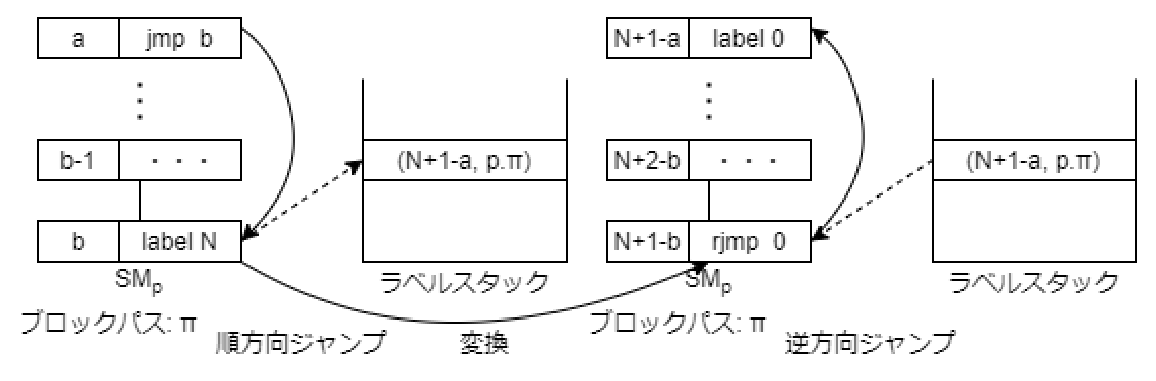
\includegraphics{jmp.eps}
%\end{figure}

逆方向の実行ではlabel命令から変換したrjmp命令でラベルスタックに積まれたジャンプ履歴を取り出しそのPCにジャンプする.ただしパスとプロセス番号が一致しているかを確認し一致していない場合実行することができない.その場合このプロセスは待ち状態となり別のプロセスが実行を進めていく.このようにして順方向の実行で起きたジャンプをちょうど逆順に辿る実行を行う.

%4.2.2
\subsubsection{変数更新履歴の利用}

図の$\sigma$は共有変数スタックを表し,$w$は演算スタックを表す.図のような方法で変数更新履歴を保存し,保存した情報を使って変数の値を逆順に戻していく.

逆方向の実行ではstore命令から変換したrestore命令で値スタックに積まれた変数の値を取り出しその値を被演算子と現在のパスが表す番地に保存することで順方向の変数の更新とは逆順に変数の値を戻す実行を行う.

\subsubsection{手続き,関数の逆方向の振る舞い}

手続き,および関数は逆方向の命令では両方ともにr\_proc命令から始まり,r\_return命令で終わる.逆方向実行では呼び出しを行った命令のPCや手続き,関数が終了して戻るPCはジャンプ履歴としてラベルスタックに保存されているため,r\_procはパスを追加する機能を持ったr\_label命令,r\_return命令はパスを削除する機能を持ったrjmp命令として動作することで逆方向の手続き,関数の実行を実現している.

\subsubsection{並列ブロックの逆方向の振る舞い}

逆方向実行ではr\_fork命令で並列ブロックを生成するために並列テーブルの参照する際,並列テーブルに保存されている各ブロックの終わりのPCおよび始まりのPCと対応する逆方向実行のバイトコードのPCをそれぞれ始まりのPCと終わりのPCとする.これによって順方向実行で生成した際と同じプロセス番号で逆方向実行でも並列プロセスを生成することができる.ネスト構造を含んでいても必ず同じプロセス番号のプロセスがネストするプロセスを生成するため順方向実行と逆方向実行のネストの構造は一致する.


%5
\section{実行例}

本章では本研究で実装した可逆実行環境の実行例を示す.\figref{fig:target}の対象プログラムを順方向実行しその実行を逆に辿る実行をすることを考える.\figref{fig:target}のプログラムは3の階乗を計算するプログラムで,関数bug\_fact(x)は再帰的に計算を行いxの階乗を返す関数である.しかしbug\_fact(x)は並列に二つのプロセスを実行し一つのプロセスは順当に階乗の計算を再帰的に行う.もう一つのプロセスは順当に行う階乗の計算を妨害するように仮引数xの値をいずれかのタイミングで1引くプロセスとなっている.この妨害プロセスがどのタイミングで行われるかによって階乗計算の結果と再帰する数及び並列プロセスの生成数が異なる例となっている.



\begin{figure}[tb]
\setbox0\vbox{
\hbox{\|begin b1|}
\hbox{\|    var x;|}
\hbox{\|    var y;|}
\hbox{\|    func f1 bug_fact(x) is|}
\hbox{\|        par a1|}
\hbox{\|            begin b2|}
\hbox{\|                var z;|}
\hbox{\|                if (x>0) then|}
\hbox{\|                    begin b3|}
\hbox{\|                        z=x-1;|}
\hbox{\|                        fact = x*{c1 fact(z)}|}
\hbox{\|                    end|}
\hbox{\|                else|}
\hbox{\|                    fact=1|}
\hbox{\|                fi|}
\hbox{\|                remove z;|}
\hbox{\|            end|}
\hbox{\|        |$||$\|  begin b4|}
\hbox{\|                if (x>1) then|}
\hbox{\|                    x = x-1|}
\hbox{\|                else|}
\hbox{\|                    skip|}
\hbox{\|                fi|}
\hbox{\|            end|}
\hbox{\|        rap|}
\hbox{\|    return|}
\hbox{\|    x=3;|}
\hbox{\|    y={c2 bug_fact(x)}|}
\hbox{\|    remove y;|}
\hbox{\|    remove x;|}
\hbox{\|end|}
}
\centerline{\fbox{\box0}}
\caption{対象プログラム(bug\_fact)}
\ecaption{a target program(bug\_fact)}
\label{fig:target}
\end{figure}


\begin{figure}[tb]
\setbox0\vbox{
\hbox{\|1 : block  b1         39: end    b2|}
\hbox{\|2 : alloc  0          40: par    1|}
\hbox{\|3 : alloc  1          41: par    0|}
\hbox{\|4 : jmp    64         42: block  b4|}
\hbox{\|5 : func   f1         43: load   0|}
\hbox{\|6 : alloc  2          44: ipush  1|}
\hbox{\|7 : alloc  0          45: op     3|}
\hbox{\|8 : store  0          46: jpc    48|}
\hbox{\|9 : fork   a1         47: jmp    54|}
\hbox{\|10: par     0         48: label  75|}
\hbox{\|11: block  b2         49: load   0|}
\hbox{\|12: alloc  3          50: ipush  1|}
\hbox{\|13: load   0          51: op     2|}
\hbox{\|14: ipush  0          52: store  0|}
\hbox{\|15: op     3          53: jmp    56|}
\hbox{\|16: jpc    18         54: label  75|}
\hbox{\|17: jmp    34         55: nop    0|}
\hbox{\|18: label  75         56: label  75|}
\hbox{\|19: block  b3         57: end    b4|}
\hbox{\|20: load   0          58: par    1|}
\hbox{\|21: ipush  1          59: merge  a1|}
\hbox{\|22: op     2          60: load   2|}
\hbox{\|23: store  3          61: free   2|}
\hbox{\|24: load   0          62: free   2|}
\hbox{\|25: load   3          63: f_return f1|}
\hbox{\|26: block  c1         64: label  75|}
\hbox{\|27: jmp    5          65: ipush  3|}
\hbox{\|28: label  75         66: store  0|}
\hbox{\|29: end    c1         67: load   0|}
\hbox{\|30: op     1          68: block  c2|}
\hbox{\|31: store  2          69: jmp    5|}
\hbox{\|32: end    b3         70: label  75|}
\hbox{\|33: jmp    37         71: end    c2|}
\hbox{\|34: label  75         72: store  1|}
\hbox{\|35: ipush  1          73: free   1|}
\hbox{\|36: store  2          74: free   0|}
\hbox{\|37: label  75         75: end    b1|}
\hbox{\|38: free    3         |}

}
\centerline{\fbox{\box0}}
\caption{順方向実行のバイトコード(bug\_fact)}
\ecaption{a byte code of forward execution(bug\_fact)}
\label{fig:forwardfact}
\end{figure}


このプログラムをコンパイラに与えることでそれぞれのステートメントを抽象機械命令に変換し順方向実行のバイトコードを生成する.\figref{fig:forwardfact}が生成した順方向実行のバイトコードである.このバイトコードを抽象機械に与えることで順方向の実行を行う.

\begin{figure}[tb]
\setbox0\vbox{
\hbox{\|0 0.b1.E|}
\hbox{\|0 0.f1.c2.b1.E|}
\hbox{\|3 0.2.b4.f1.c2.b1.E|}
\hbox{\|0 0.1.b3.b2.f1.c2.b1.E|}
\hbox{\|0 0.1.f1.c1.b3.b2.f1.c2.b1.E|}
\hbox{\|2 0.1.2.b4.f1.c1.b3.b2.f1.c2.b1.E|}
\hbox{\|0 0.1.1.b3.b2.f1.c1.b3.b2.f1.c2.b1.E|}
\hbox{\|0 0.1.1.f1.c1.b3.b2.f1.c1.b3.b2.f1.c2.b1.E|}
\hbox{\|0 0.1.1.1.b3.b2.f1.c1.b3.b2.f1.c1.b3.b2.f1.c2.b1.E|}
\hbox{\|0 0.1.1.1.f1.c1.b3.b2.f1.c1.b3.b2.f1.c1.b3.b2.f1.c2.b1.E|}
\hbox{\|0 0.1.1.1.1.b2.f1.c1.b3.b2.f1.c1.b3.b2.f1.c1.b3.b2.f1.c2.b1.E|}
\hbox{\|0 0.1.1.1.b3.b2.f1.c1.b3.b2.f1.c1.b3.b2.f1.c2.b1.E|}
\hbox{\|0 0.1.1.b3.b2.f1.c1.b3.b2.f1.c2.b1.E|}
\hbox{\|0 0.1.b3.b2.f1.c2.b1.E|}
\hbox{\|0 0.b1.E|}
}
\centerline{\fbox{\box0}}
\caption{値スタック(bug\_fact)}
\ecaption{value stack(bug\_fact)}
\label{fig:value}
\end{figure}

\begin{figure}[tb]
\setbox0\vbox{
\hbox{\|72 0.b1.E|}
\hbox{\|7 0.c2.b1.E|}
\hbox{\|30 0.2.b4.f1.c2.b1.E|}
\hbox{\|60 0.1.b2.f1.c2.b1.E|}
\hbox{\|23 0.2.b4.f1.c2.b1.E|}
\hbox{\|49 0.1.c1.b3.b2.f1.c2.b1.E|}
\hbox{\|60 0.1.1.b2.f1.c1.b3.b2.f1.c2.b1.E|}
\hbox{\|30 0.1.2.b4.f1.c1.b3.b2.f1.c2.b1.E|}
\hbox{\|23 0.1.2.b4.f1.c1.b3.b2.f1.c2.b1.E|}
\hbox{\|49 0.1.1.c1.b3.b2.f1.c1.b3.b2.f1.c2.b1.E|}
\hbox{\|60 0.1.1.1.b2.f1.c1.b3.b2.f1.c1.b3.b2.f1.c2.b1.E|}
\hbox{\|29 0.1.1.2.b4.f1.c1.b3.b2.f1.c1.b3.b2.f1.c2.b1.E|}
\hbox{\|21 0.1.1.2.b4.f1.c1.b3.b2.f1.c1.b3.b2.f1.c2.b1.E|}
\hbox{\|49 0.1.1.1.c1.b3.b2.f1.c1.b3.b2.f1.c1.b3.b2.f1.c2.b1.E|}
\hbox{\|59 0.1.1.1.1.b2.f1.c1.b3.b2.f1.c1.b3.b2.f1.c1.b3.b2.f1.c2.b1.E|}
\hbox{\|29 0.1.1.1.2.b4.f1.c1.b3.b2.f1.c1.b3.b2.f1.c1.b3.b2.f1.c2.b1.E|}
\hbox{\|21 0.1.1.1.2.b4.f1.c1.b3.b2.f1.c1.b3.b2.f1.c1.b3.b2.f1.c2.b1.E|}
\hbox{\|40 0.1.1.1.1.b2.f1.c1.b3.b2.f1.c1.b3.b2.f1.c1.b3.b2.f1.c2.b1.E|}
\hbox{\|13 0.1.1.1.c1.b3.b2.f1.c1.b3.b2.f1.c1.b3.b2.f1.c2.b1.E|}
\hbox{\|43 0.1.1.1.b2.f1.c1.b3.b2.f1.c1.b3.b2.f1.c2.b1.E|}
\hbox{\|13 0.1.1.c1.b3.b2.f1.c1.b3.b2.f1.c2.b1.E|}
\hbox{\|43 0.1.1.b2.f1.c1.b3.b2.f1.c2.b1.E|}
\hbox{\|13 0.1.c1.b3.b2.f1.c2.b1.E|}
\hbox{\|43 0.1.b2.f1.c2.b1.E|}
\hbox{\|13 0.c2.b1.E|}
}
\centerline{\fbox{\box0}}
\caption{ラベルスタック(bug\_fact)}
\ecaption{label stack(bug\_fact)}
\label{fig:label}
\end{figure}



\figref{fig:forwardfact}を抽象機械で実行すると\figref{fig:value},\figref{fig:label}のように値スタック,ラベルスタックに逆方向実行に必要な情報が保存される.\figref{fig:value}は値スタックを示し,一行のうち左側に変数の値,右側にstore命令を行ったプロセスとパスが保存されている.例えば一行目の(0 0.b1.E)はプロセス0のパスb1の状態で何らかの変数の値を更新しその変数のそれまでの値が0であったことを示す.プロセス0.1,プロセス0.2は並列で動作しているプロセスだが三行目,四行目を見るとその実行順がプロセス0.2,プロセス0.1の順番で実行されたことが保存されている.
\figref{fig:label}はラベルスタックを示し,一行のうち左側にジャンプしたPCの値,右側にlabel命令を行ったプロセスとパスが保存されている.例えば一行目の(72 0.b1.E)はプロセス0のパスb1の状態でPC=72の命令からlabel命令にジャンプしてきたことを示す.特に条件分岐について条件判定を行わずともどこから分岐(ジャンプ)したかという情報が残されているためラベルスタックを見るだけでどのように分岐したかがわかる.






\begin{figure}[tb]
\setbox0\vbox{
\hbox{\|1 : block   b1         39: rjmp    0|}
\hbox{\|2 : r_alloc 0          40: restore 2|}
\hbox{\|3 : r_alloc 1          41: nop     0|}
\hbox{\|4 : restore 1          42: rjmp    0|}
\hbox{\|5 : block   c2         43: r_label 0|}
\hbox{\|6 : rjmp    0          44: block   b3|}
\hbox{\|7 : r_label 0          45: restore 2|}
\hbox{\|8 : end     c2         46: nop     0|}
\hbox{\|9 : nop     0          47: block   c1|}
\hbox{\|10: resotre 0          48: rjmp    0|}
\hbox{\|11: nop     0          49: r_label 0|}
\hbox{\|12: rjmp    0          50:  end    c1|}
\hbox{\|13: r_proc  f1         51: nop     0|}
\hbox{\|14: r_alloc 2          52: nop     0|}
\hbox{\|15: r_alloc 0          53: restore 3|}
\hbox{\|16: nop     0          54: nop     0|}
\hbox{\|17: r_fork  a1         55: nop     0|}
\hbox{\|18: par     0          56: nop     0|}
\hbox{\|19: block   b4         57: end     b3|}
\hbox{\|20: rjmp    0          58: rjmp    0|}
\hbox{\|21: nop     0          59: r_label 0|}
\hbox{\|22: rjmp    0          60: r_label 0|}
\hbox{\|23: r_label 0          61: nop     0|}
\hbox{\|24: restore 0          62: nop     0|}
\hbox{\|25: nop     0          63: nop     0|}
\hbox{\|26: nop     0          64: free    3|}
\hbox{\|27: nop     0          65: end     b2|}
\hbox{\|28: rjmp    0          66: par     1|}
\hbox{\|29: r_label 0          67: merge   a1|}
\hbox{\|30: r_label 0          68: restore 0|}
\hbox{\|31: nop     0          69: free    0|}
\hbox{\|32: nop     0          70: free    2|}
\hbox{\|33: nop     0          71: r_return f1|}
\hbox{\|34: end     b4         72: r_label 0|}
\hbox{\|35: par     1          73: free    1|}
\hbox{\|36: par     0          74: free    0|}
\hbox{\|37: block   b2         75: end     b1|}
\hbox{\|38: r_alloc 3         |}

}
\centerline{\fbox{\box0}}
\caption{逆方向実行のバイトコード(bug\_fact)}
\ecaption{a byte code of backward execution(bug\_fact)}
\label{fig:backwardfact}
\end{figure}


\figref{fig:forwardfact}の抽象命令を一対一で変換し順番を反転させたものが\figref{fig:backwardfact}である.変数の宣言,更新,解放やジャンプやパスの追加,削除そして並列ブロックに関わる命令以外は全てnopに変換されている.これは本研究における逆方向実行は変数の値を元に戻すということを主目的としているためである.そのため演算スタックを元に戻すという動作が存在しない.

\figref{fig:backwardfact}の逆方向実行バイトコードと\figref{fig:value},\figref{fig:label}の逆方向実行に必要な情報を用いて順方向の実行を逆方向に辿る.\figref{fig:value}と\figref{fig:label}の下から保存した情報を消費していく.それぞれrestore命令とrjmp命令においてパスが一致しているか否かを判定し一致している場合左側の値を消費して変数の値を戻したりジャンプを逆方向に辿っていく.パスが一致していない場合そのプロセスの実行は待ち状態になり別プロセスが実行を進める.このようにして順方向で実行した順番とちょうど逆順に変数の更新と逆方向ジャンプを行う.



%6
\section{おわりに}





\end{document}
